\documentclass[12pt]{article}
\usepackage{hyperref}
\usepackage{amsmath, amssymb, amsfonts}
\usepackage[margin=2cm]{geometry}
\usepackage{xcolor}
\usepackage{graphicx}
\usepackage{xparse}
\usepackage{enumitem, inconsolata}
\parindent 0px
\newcommand{\W}{\(\Omega\)}
\newcommand{\w}{\(\omega\)}
\newcommand{\lb}{\\$\left|\rightarrow\right.$}
\newcommand{\enter}{\\\textcolor{white}{1}}
\ExplSyntaxOn
\newcommand{\sub}[1]{\textsubscript{#1}}
\newcommand{\super}[1]{\textsuperscript{#1}}

\NewDocumentCommand{\bo}{m}
 {
   \bold_commas:n { #1 }
 }

\cs_new:Npn \bold_commas:n #1
 {
   \seq_set_split:Nnn \l_tmpa_seq { , } { #1 }
   \seq_map_indexed_function:NN \l_tmpa_seq \__bold_commas_aux:nn
 }

\cs_new:Npn \__bold_commas_aux:nn #1 #2
 {
   \textbf{#2}
   \int_compare:nNnTF { #1 } < { \seq_count:N \l_tmpa_seq }
     { , }
     { }
 }

\ExplSyntaxOff

\title{Operating System}
\author{Me lol}
\date{\today}

\begin{document}
\maketitle
\vspace{13cm}
\begin{large}\textbf{Notes}\end{large}
\begin{itemize}
\item PYQs of BEI's CT612, BCT's CT656, BCT's EX652 and BCT's EG682CT are combined.
\item BEI's CT612 questions' markings are \texttt{stylized with this font for clarity}.
\item The marking of questions of 66 Magh is \bo{not} \bo{given}. All marking given in this collection are \bo{assumed} marks based on other pyq's. 
\end{itemize}
\pagebreak
\tableofcontents
\pagebreak

\section{Introduction}
	\begin{center}(5 Hours/10 Marks)\end{center}
	\subsection{Operating System and Function}
	\begin{enumerate}
	\item Define operating system.\hfill[1] \begin{footnotesize}(\bo{\texttt{80 Bh}, 80 Ch, 79 Ch, 76 Bh}, 76 Ba, 75 Ba, \bo{72 Ash}, 71 Ma, 65 Ka)\end{footnotesize}
	\item Explain the functions of Operating System.\hfill[3] \begin{footnotesize}(\bo{76 Bh}, 75 Ba, 73 Ma, \bo{68 Bh})\end{footnotesize} [4] \begin{footnotesize}(\bo{72 Ash})\end{footnotesize} 
	\lb What are the primary purposes of an operating system? Explain.\hfill[3] (\bo{73 Bh})
	\item How does operating system provide a beautiful interface to user?\hfill[3] (\bo{\texttt{81 Bh}})
	\item Justify how OS act as resource manager.\hfill[3]\begin{small} (\texttt{81 Ba}, \bo{77 Ch}, 76 Ba)\end{small} [4]\begin{small} (68 Ma, 65 Ka)\end{small}
	\item Explain the statement: Operating system acts as a broker between hardware and application program.\hfill[4] (\bo{\texttt{80 Bh}, 79 Ch})
	\item Explain OS as an Extended Machine.\hfill[2] (\texttt{80 Ba}, 70 Ma)
	\lb How does an OS create abstraction? Explain with reference to OS as an extended machine.\hspace{13.4cm}[5] (\bo{69 Bh})
	\item Explain the virtual machine structure. What are the benefits over other operating system architecture?\hfill[2+2] (\bo{74 Bh, 72 Ash})
	\item Why Operating system is termed as virtual machine?\hfill[2] (73 Ma)
	\lb Explain operating system as a virtual machine.\hfill[2] (\bo{67 Mng}) [4] (\texttt{80 Ba})

	\item Why should the operating system prevent users from accessing the boot sector?\hfill[2] (\bo{73 Bh})
	\item Explain in detail about context switching.\hfill[4] (\bo{67 Mng})
	\item What features does an operating system expose on top of the hardware to enhance user experience? Explain. \hfill[8] (\bo{66 Ma})
	\end{enumerate}
	\subsection{Evolution of Operating System}
	\begin{enumerate}
	\item Why operating system evolve over long periods of time?\hfill[1] (\texttt{81 Ba})
	\end{enumerate}
	\subsection{Type of Operating System: Batch, Interactive, Multiprocessing, Time Sharing and Real Time System}
	\begin{enumerate}
	\item Explain in brief any four types of OS.\hfill[5] (\bo{73 Bh})
	\lb Briefly mention the type of operating system.\hfill[4] (71 Ma)
	\item List the essential properties for the Batch-oriented and Interactive operating system.
	\enter\hfill[4] (\bo{70 Bh})
	\item Write down the major differences between following types of operating system.
	\enter\hfill[8] (\bo{78 Ch, 71 Bh})\\
	a. Batch system\hspace{7mm}b. Interactive system\hspace{7mm}c. Real time system\hspace{7mm}d. Time sharing system
	\item Discuss the properties of batch system and real time system.\hfill[4] (76 Ba)
	\item Explain multiprogramming, multiprocessing and distributed operating system.\hfill[6] (74 Bh)
	\item For each of the following application which system (Batch or Interactive) is more suitable?\\
	a. Word Processing \hspace{5cm}b. A flight simulator\hfill[6] (\bo{70 Bh})\\
	c. Computing pi to million decimal places\hspace{9mm} d. Generating monthly bank statements\\ 
	e. Generating mark statement by University \hspace{7mm}f. Data acquisition from temperature sensor
	\end{enumerate}
	\subsection{Operating System Components}
	\begin{enumerate}
	\item What do you understand by firmware? Can you relate with operating system? Are there any linkages among hardware, software, firmware and operating system?\hfill[10] (70 Ma)
	\end{enumerate}
	\subsection{Operating System Structure: Monolithic, Layered, Micro-Kernel, Client-Server, Virtual Machine}
	\begin{enumerate}
	\item What are the different structures of an operating system?\hfill[2] (\bo{67 Mng})
	\item Why Exo-Kernel doesn't require Re-mapping of resources?\hfill[2] \begin{small}(\bo{\texttt{81 Bh}, 79 Ch})\end{small} [3] \begin{small}(\bo{80 Ch})\end{small}
	\item Is layered structure of operating system is better than monolithic structure? Explain.
	\enter \hfill[3] \begin{small}(\bo{\texttt{81 Bh}, 79 Ch})\end{small} [4] \begin{small}(\bo{80 Ch})\end{small} [10] \begin{small}(72 Ma)\end{small}
	\item Differentiate between Monolithic Kernel and Micro-Kernel.\hfill[4] (\texttt{80 Ba}) [5] (71 Ma)
	\item Distinguish between kernel and micro-kernel.\hfill[3] (70 Ma)
	\item Explain about microkernel.\hfill[5] (\bo{68 Bh})
	\item Explain the Monolithic and layered architecture of operating system. Explain which architecture is better among them and why?\hspace{6.7cm}[2+1] (\bo{76 Bh})\\
	\lb Explain in brief about monolithic architecture and virtual machine.\hfill[3] (73 Ma)
	\item Discuss about Microkernel and Monolithic structuring with their adv and disadv.[3] (\bo{77 Ch}) 
	\item Why is the process table needed in a timesharing system? Is it also needed in personal computer systems running UNIX or Windows with a single user?\hfill[6] (\bo{\texttt{79 Bh}})
	\item Distinguish between Shell and Kernel.\hfill[4] (\bo{\texttt{79 Bh}})
	\end{enumerate}
	\subsection{Operating System Services}
	\subsubsection{System calls}
	\begin{enumerate}
	\item What is system call in OS?\hfill[1] \begin{small}(\bo{77 Ch, 76 Bh}, 75 Ba)\end{small} [2] \begin{small}(73 Ma)\end{small}
	\item What is the purpose of a system call in an operating system?
	\enter\hfill[2] \begin{small}(\bo{78 Ch, 71 Bh})\end{small} [3] \begin{small}(\bo{80 Ch}, 70 Ma)\end{small}
	\item Define system call and explain its working mechanism with suitable example.\hfill[5] (\bo{69 Bh})
	\item Illustrate the execution of system call read() to read a file.\hfill[5] (75 Ba)
	\end{enumerate}
	\subsubsection{Shell commands}
	\begin{enumerate}
	\item What do you mean by Shell?\hfill[1] (\bo{77 Ch})
	\item What is pipe and shell?\hfill[4] (68 Ma)
	\end{enumerate}
	\subsubsection{Shell programming}
	\begin{enumerate}
	\item Write short notes on Shell Programming.\hfill[4] (\bo{75 Bh})
	\end{enumerate}

	\pagebreak
\section{Process Management}
	\begin{center}(6 Hours/10 Marks)\end{center}
	\subsection{Introduction to Process }
	\begin{enumerate}[noitemsep, topsep = 0pt]
		\item Define process. \hfill [1] (\bo{75 Bh}, 73 Ma) [2] (71 Ma)
		
		\item (Assumed:) What is dispatcher? \hfill [1] (\bo{67 Mng})
	\end{enumerate}
	
	\subsubsection{Process description}
	\begin{enumerate}
		\item What is priority of a process? Why do we need it? Explain. \hfill [2] (\bo{\texttt{80 Bh}})
	\end{enumerate}
	
	\subsubsection{Process states}
	\begin{enumerate}[noitemsep, topsep=0pt]
		\item Describe the various states of process.\hfill [1] (\bo{75 Bh}) [2] (73 Ma)
		\lb Discuss 5-state model of process. \hfill [3] (\bo{71 Bh})
	\end{enumerate}
	
	\subsubsection{Process control}
	\begin{enumerate}[noitemsep, topsep = 0pt]
		\item Explain fork() and spawn() system calls in the OS. \hfill [3] (\texttt{81 Ba})
		
		\item Explain Context Switching with an example. \hfill [2] (\texttt{80 Ch})
		
		\item What is Process Control Block? \hfill [2] (\bo{69 Bh})		
		
		\item What information does a process control block contain? \hfill [3] (\bo{79 Ch})
		
		\item How significant is the process hierarchy? \hfill [2] (73 Ma)
	\end{enumerate}
	
	\subsection{Threads}
	\begin{enumerate}[noitemsep, topsep = 0pt]
		\item Explain the advantages of multithreading. \hfill [2] (\bo{72 Ash})
	\end{enumerate}
	\subsection{Processes and Threads}
	\begin{enumerate}[noitemsep, topsep = 0pt]
		\item Define Process and Threads. \hfill [2] (\bo{76 Bh})
		
		\item Write the difference between thread and process. 
		\enter\hfill [1] (\bo{77 Ch}) [2] (\bo{79 Ch, 74 Bh, 72 Ash}, 76 Ba) [3] (\bo{67 Mng}, 72 Ma)
		
		\item Why threads are called light weight process? \hfill [2] (\bo{\texttt{81 Bh}})
		
		\item What is multithreading? Explain five state process model with figure. \hfill [4] (\texttt{80 Ba})
		
		\item State 5-State process model. \hfill [2] (\bo{78 Ch})
		
		\item What are the advantages and disadvantages of implementing threads in user space?
		\enter \hfill [4] (\bo{\texttt{79 Ch}})
		
		\item Define Context Switching. \hfill [2] (\bo{71 Bh})
		
		\item Explain how thread based execution minimizes context switching problem of process based execution. \hfill [2] (\bo{74 Bh})
		
		\item Explain how multi threading provide better solution than single threading solution.
		\enter \hfill [3] (\bo{77 Ch})
	\end{enumerate}
	\subsubsection{Types of scheduling}
	\begin{enumerate}[noitemsep, topsep = 0pt]
		\item Differentiate between Preemptive and Non-Preemptive Scheduling. \hfill [2] (\texttt{80 Ba}) [4] (\bo{68 Bh})
		
		\item What is real time scheduling? \hfill [2] (75 Ba)
	\end{enumerate}
	\subsubsection{Scheduling in Interactive System}
	\begin{enumerate}[noitemsep, topsep = 0pt]
		\item Explain scheduling algorithms in interactive system. \hfill [8] (\bo{69 Bh})
	\end{enumerate}
	\subsubsection{Numericals}
	\begin{enumerate}
		\item Consider the following set of processes, with length of the CPU burst time given in milliseconds. \hfill [8] (\bo{\texttt{81 Bh}, 77 Ch})\\
		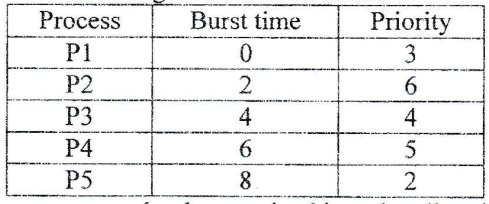
\includegraphics[width=3.5in]{os_1}\\
		A. All the processes are assumed to have arrived in order all at time 0.
		\begin{enumerate}[noitemsep, topsep = 0pt, label = \alph*.]
			\item Draw Gantt Chart Using FCFS, SJF scheduling algorithm.
			\item Find average turnaround time for each scheduling algorithm.
		\end{enumerate}
		B. Draw Gantt chart illustrating RR (quantum = 2) and highest ratio next (HRN) scheduling. Also find average waiting and average turn around time for each of the algorithm.
		
		\item Schedule the following set of process according to Round-Robin scheduling algorithm with Quantum time = 4ms and calculate the average waiting time and average Turn-around time, throughput and CPV utilization. \hfill [3] (\texttt{81 Ba})\\
		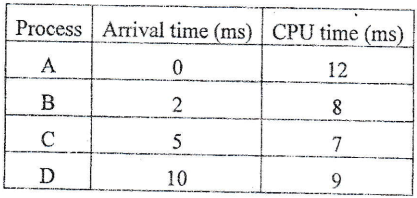
\includegraphics[width=3.5in]{os_2}
		
		\item Consider the following set of processes, with length of the CPU burst time given in milliseconds. \hspace{12.9cm} [8] (\bo{80 Ch})\\
		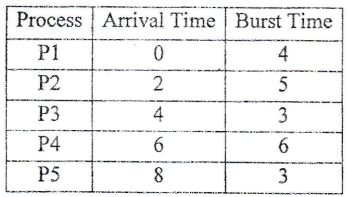
\includegraphics[width=3.5in]{os_3}\\
		With all the given information, draw the Gantt Chart and calculate the average waiting time (AWT), average turnaround time (ATAT), CPU utilization and throughput for the
		\begin{enumerate}[noitemsep, topsep = 0pt, label = \alph*.]
			\item Round Robin (RR) (Quantum Time = 2)
			\item Highest Response Ratio Next (HRRN)
		\end{enumerate}
		
		\item Make  schedule for the processes mentioned in the table below as per Shortest Remaining Time First (SRTF) algorithm. Also calculate average turnaround time and average waiting time, throughput and CPU utilization. \hfill [6] (\bo{\texttt{80 Bh}})
		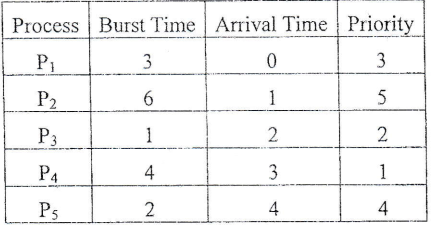
\includegraphics[width=3.5in]{os_4}
		
		\item Apply MLQ scheduling for following set of processes of two queues Q1 and Q2 where Priority of Q1 is greater than that of Q2 and Q1 uses Round Robin (Time Quantum = 2) and Q2 uses FCFS. Construct Gantt-Chart and computer average TAT for above scenario.
		\enter \hfill [4] (\texttt{80 Ba})\\
		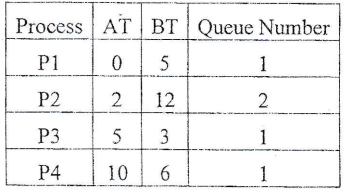
\includegraphics[width=3.5in]{os_5}
		
		\item Consider following set of process with given arrival and CPU burst time. Calculate the average waiting time for each of process for non-primitive shortest job first (SJF) and Round Robin Scheduling Algorithms with quantum size 4. \hfill [5] (\bo{79 Ch})\\
		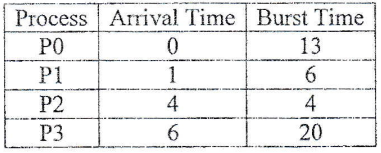
\includegraphics[width=3.5in]{os_6}
		
		\item Consider the following set of processes, with arrival time and the length of CPU burst time given in millisecond as below: \hfill [6] (76 Ba)\\
		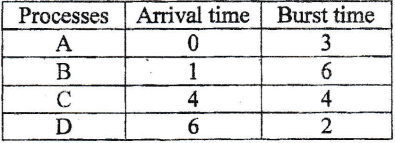
\includegraphics[width=3.5in]{os_10}\\
		\begin{enumerate}[noitemsep, topsep = 0pt, label = \alph*.]
			\item Draw Gantt chart illustrating the execution of these processes using FCFS, SRTN and RR (Quantum = 2) scheduling.
			\item What is the waiting time and Turnaround time of each process for each of th escheduling algorithm?
		\end{enumerate}
		
		\item Let us consider five process with given arrival time and length of the CPU burst given in milliseconds. Calculate the turnaround time and waiting time for all processes applying First Come First Serve, Shortest Job first and Round Robin (time quantum = 3) algorithms.\\
		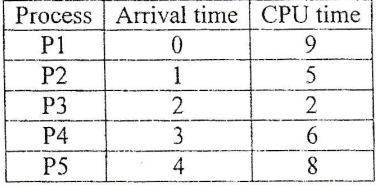
\includegraphics[width=3.5in]{os_8}
		\hfill [6] (\bo{\texttt{79 Bh}})
		
		\item Assume the process arrived in the order p\sub{1}, p\sub{2}, p\sub{3}, p\sub{4} and p\sub{5} all time 0, priority 1 as highest and 4 as lowest. \hfill [8] (\bo{78 Ch})\\
		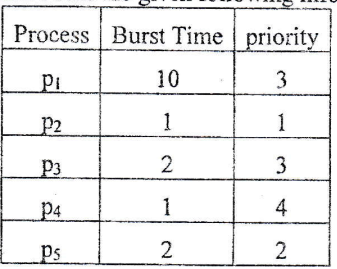
\includegraphics[width=2in]{os_7}
		\begin{enumerate}[noitemsep, topsep = 0pt, label = \alph*.]
			\item Draw the gantt chart
			\item Calculate average waiting time and average turnaround for the following scheduling algorithm.\\
			i. Round robin (quantum = 1)\\
			ii. priority preemptive\\
			iii. preemptive SJF\\
			iv. FCFS
		\end{enumerate}
		
		\item Consider the following processes, with the length of the CPU burst time in millisecond. The processes are assumed to have arrived in the order P1, P2, P3, P4, P5 all at time 0. [Lowest number being Highest Priority] \hfill [6] (\bo{75 Bh})\\
		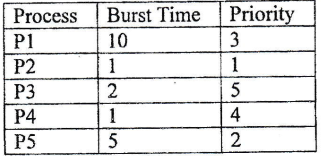
\includegraphics[width=3.5in]{os_11}\\
		Draw Gantt chart illustrating priority and RR (quantum = 1) scheduling. Also find average waiting time and average turn-around time for each of the algorithms.
		
		\item Consider the following set of processes, with arrival time and the length of CPU burst time given in millisecond as below: \hfill [4+4] (\bo{76 Bh})\\
		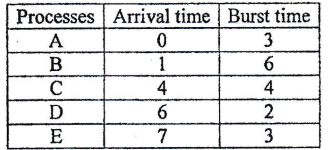
\includegraphics[width=3.5in]{os_9}
		\begin{enumerate}[noitemsep, topsep = 0pt, label = \alph*.]
			\item Draw Gantt chart illustrating the execution of these processes using FCFS, SRTN and RR (Quantum = 3) scheduling.
			\item What is the waiting time and Turnaround time of each process for each of the scheduling algorithm?
		\end{enumerate}
		
		\item Consider the following set of processes, with the length of the burst time given in milliseconds: (Assume the system has two processors P\sub{1} and P\sub{2}). \hfill [8] (75 Ba)\\
		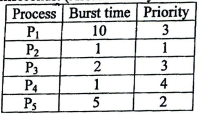
\includegraphics[width=3.5in]{os_12}\\
		The processes are assumed to have arrived in order p1, p2, p3, p4, p5 all at time 0. Compute the AWT and ATAT for each of the scheduling algorithms. (1) FCFS (2) SJF (3) Pre-emptive priority (4) RR (q=1) scheduling.
		
		\item Suppose 5 processes are submitted at time 0.\\
		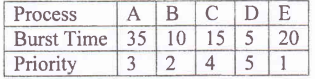
\includegraphics[width=3.5in]{os_13}\\
		Show the execution timeline of the process using Gantt Chart for FCFS, SJF and Round Robin (q=5). Also calculate mean turnaround time in each case. \hfill [6] (\bo{74 Bh})
		
		\item Make a schedule as per Rate Monotonic (RM) algorithm for the following set of real time tasks:\hfill [5] (73 Ma)\\
		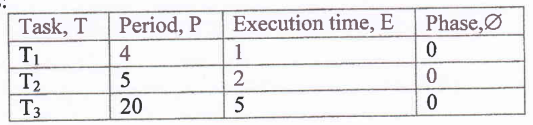
\includegraphics[width=3.5in]{os_14}
		
		\item Assume the system having two processors of same configuration, schedule the following set of processes according to preemptive priority and round robin algorithm (quantum = 3) and calculate average waiting time and average turnaround time. \hfill [5+5] (\bo{73 Bh})
		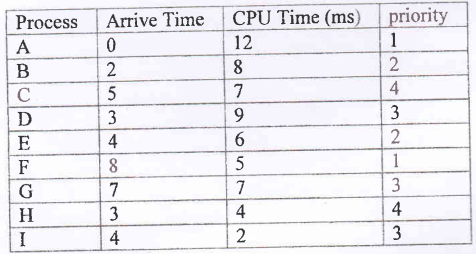
\includegraphics[width=3.5in]{os_15}
		
		\item Assume you have the following processes to execute with one processor. \hfill [5] (72 Ma)\\
		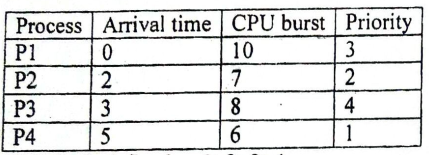
\includegraphics[width=3.5in]{os_16}\\
		Priority is defined as \( 1 > 2 > 3 > 4 \)\\
		i) Make the GANTT chart of the execution of these using preemptive priority and shortest remaining time first algorithm.\\
		ii) Find out turnaround time, waiting time, and their average time of each process.
		
		\item Schedule the following set of processes according to HRRN and Round Robin algorithm (Time quantum = 4) and calculate average waiting time and average turnaround time. 
		\enter\hfill [5] (\bo{72 Ash})\\
		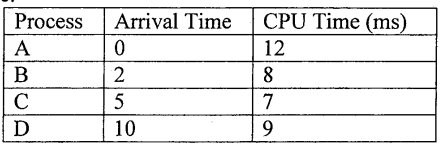
\includegraphics[width=3.5in]{os_17}
		
		\item From the given following information: \hfill [5] (71 Ma)\\
		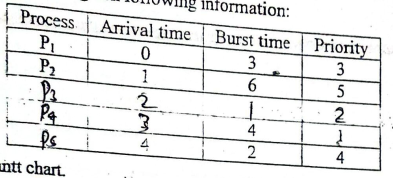
\includegraphics[width=3.5in]{os_18}\\
		a) Draw the Gantt Chart.\\
		b) Calculate average waiting time and average turn around time for the following scheduling algorithm.\\
		i) Round Robin (q=1) \hspace{1cm} ii) Priority Preemptive \hspace{1cm} iii) Preemptive SJF
		
		\item Schedule the following set of process according to multilevel feedback queue scheduling algorithm and compute AWT and ATAT. \hfill [5] (\bo{71 Bh})\\
		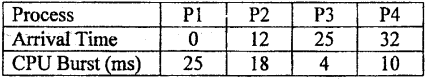
\includegraphics[width=3.5in]{os_19}\\
		Assume that there are three ready queues Q1, Q2 and Q3. The CPU time slice for Q1 and Q2 is 5 ms and 10 ms respectively and processes are scheduled on FCFS basis in Q3.
		
		\item For the process listed in following table, what is the average turnaround time using: \\
		a) FCFS \hspace{6mm} b) RR (quantum = 4) \hspace{6mm} c) SJF \hspace{6mm} d) SRT \hspace{6mm} e) HRRN \hfill [10] (70 Ma)\\
		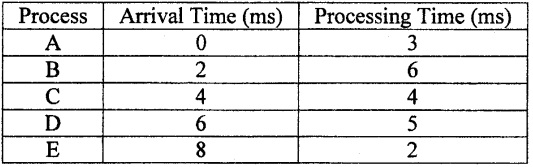
\includegraphics[width=3.5in]{os_20}
		
		\item Consider the following set of process with the length of the CPU burst time given in millisecond. \hfill [4+4] (\bo{70 Bh})
		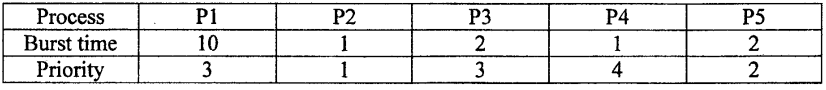
\includegraphics[width=6in]{os_21}\\
		Assume the processes arrived in the order P1, P2, P3, P4 and P5 all at time 0, priority 1 as highest and 4 as lowest.\\
		a. Draw the Gantt chart for FCFS, SJF, Priority and Round Robin (Quantum = 2)\\
		b. Which algorithm results in the maximum average waiting time?
		
		\item Assume you have the following jobs to execute with one processor. \hfill [6] (68 Ma)\\
		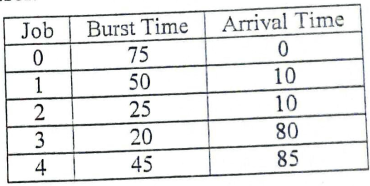
\includegraphics[width=3.5in]{os_22}\\
		Suppose a system uses round-robin scheduling with quantum of 15 sec.\\
		a. Draw the Gantt chart.\\
		b. Find the average wait and turnaround time.
		
		\item A system that uses the Banker's Algorithm deadlock avoidance has five processes (1, 2, 3, 4, 5) and four types of resources (A, B, C and D). There are multiple resoures ofeach type. Is the following state safe or not? If it is, show how the process can complete. If not, show how they can deadlock. \hfill [8] (\bo{68 Bh})\\
		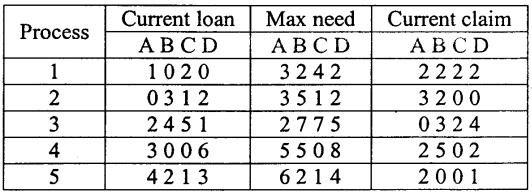
\includegraphics[width=3.5in]{os_23}\\
		Resources Available \hspace{1cm} Total Resources\\
		A B C D \hspace{3cm} A B C D\\
		3\hspace{3mm}4\hspace{2mm}0\hspace{2mm}1\hspace{3.1cm} 13 13 9 13
		
		\item Schedule the following process applying highest response ratio hext scheduling algorithm. Assume P\sub{1} is the first process. If P\sub{4} need 2 second of service time does the sequence of schedule change? \hfill [7] (\bo{67 Mng})\\
		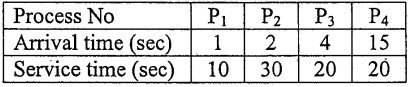
\includegraphics[width=3.5in]{os_24}
	\end{enumerate}
	
	\subsection{Multiprocessor Scheduling concept}

	\pagebreak
\section{Process Communication and Synchronization}
\begin{center}(5 Hours/10 Marks)\end{center}
	\subsection{Principles of Concurrency}
		\begin{enumerate}[noitemsep, topsep=0pt]
			\item What is the need process synchronization? \hfill [2] (\bo{\texttt{80 Bh}}, \texttt{80 Ba}, 72 Ma)
		\end{enumerate}
		
	\subsection{Critical Region}
		\begin{enumerate}[noitemsep, topsep=0pt]
			\item Define critical section with respect to multiple-process system. \hfill [1.5] (70 Ma)
			\lb What is critical section. \hfill [1] (\bo{65 Ch})
			
			\item What is Critical Section Problem? \hfill [2] (\bo{80 Ch, 78 Ch, 75 Bh, 73 Bh, 70 Bh}, 76 Ba)
			
			\item Explain how Sleep() and Wakeup() solution is better than busy waiting solution for critical section problem. \hfill [3] (\bo{79 Ch, 74 Bh})
			
			\item Why do we need pipe() function? \hfill [3] (71 Ma)
			
			\item Why is it important for a thread to execute a critical section as quickly as possible? \hfill [3] (\bo{73 Bh})
		\end{enumerate}
		
	\subsection{Race Condition}	
		\begin{enumerate}[noitemsep, topsep=0pt]
			\item Define race condition? \hfill [1] (\bo{79 Ch}, 75 Ba) [2] (\bo{79 Bh, 74 Bh, 70 Bh}, 73 Ma)
			\lb with example. \hfill [3] (\bo{71 Bh})

			\item How does a race condition arrive in IPC? \hfill [2] (\bo{77 Ch})
			
			\item What requirements should be met by race condition's solution? \hfill [2] (76 Ba) [3] (75 Ba)
			
			\item Disabling interrupts may help avoid race conditions. Explain its drawbacks as well.
			\enter\hfill [8] (\bo{66 Ma})
			
			\item Explain Peterson's solution to avoid race condition. \hfill [4] (76 Ba)
			\lb Explain Peterson's Solution. \hfill [4] (72 Ma)
			\lb Explain Peterson's Algorithm. \hfill [7] (\bo{71 Bh})
		\end{enumerate}
		
	\subsection{Mutual Exclusion}
		\begin{enumerate}[noitemsep, topsep=0pt]
			\item What is Mutual Exclusion? \hfill [1] (\bo{79 Ch}, 75 Ba, 65 Ch) [2] (\bo{\texttt{79 Bh}})
			
			\item Define critical section with respect to multiple-process system. \hfill [1.5] (70 Ma)
			
			\item Why must the executing the critical section be mutually exclusive? \hfill [2] (\bo{78 Ch, 75 Bh})
			
			\item What are the requirements of mutual exclusion? \hfill [2] (\bo{\texttt{79 Ch}}, 73 Ma)
			\lb What are conditions to get mutual exclusion? \hfill [2] (\bo{69 Bh})
			
			\item Explain about lock variable for achieving Mutual Exclusion. \hfill [2] (\bo{\texttt{81 Bh}})
			
			\item Explain Peterson's Solution in mutual exclusion. \hfill [3] (\texttt{80 Ba}) [6] (\bo{\texttt{79 Bh}})
		\end{enumerate}
		
	\subsection{Semaphores and Mutex}
		\begin{enumerate}[noitemsep, topsep=0pt]			
			\item What is is Semaphore? \hfill [1] (\bo{73 Bh, 69 Bh}, \texttt{80 Ba}, 65 Ka)

			\item How semaphore is used in process synchronization? \hfill [1] (\bo{79 Ch}, \texttt{81 Ba})
			
			\item What is the use of semaphores in interprocess communication. Explain with a suitable example. \hfill [2] (65 Ka)
			
			\item Explain major operations in semaphore. \hfill [4] (71 Ma)
			\lb including pseudocode. \hfill [5] (\bo{73 Bh})
			
			\item How can semaphore be used to enforce mutual exclusion? Give example. \hfill [5] (75 Ba)
			
			\item Describe how semaphore can be used to solve the critical section problem. \hfill [4] (\bo{75 Bh})
			
			\item Explain the major operations of semaphore with a simple implementation as a class.
			\enter\hfill [3] (\bo{74 Bh})
			
			\item Explain the types of semaphore along with major operations of semaphore with a simple pseudocode. \hfill [5] (\bo{\texttt{81 Bh}})
			
			\item Can semaphores be used in distributed system? Explain why or why not? \hfill [3] (71 Ma)
		\end{enumerate}
		
	\subsection{Test and Set Lock}
		\begin{enumerate}[noitemsep, topsep=0pt]
			\item What is TSL? \hfill [1] (\bo{74 Bh})
			\lb What is TSL instruction? \hfill [2] (\bo{72 Ash})
			
			\item Why is TSL used? \hfill [1] (\bo{74 Bh})
			\lb Why is TSL instruction used? \hfill [2] (\bo{72 Ash})
			
			\item Explain TSL instruction approaches used in mutual exclusion with busy waiting.
			\enter\hfill [4] (72 Ma)
		\end{enumerate}
		
	\subsection{Message Passing}
		\begin{enumerate}[noitemsep, topsep=0pt]
			\item Solve producer consumer problem using semaphore and emssage passing. \hfill [6] (73 Ma)
			
			\item What makes the message passing IPC as one among the best method of IPC implementation? Explain with pseudo code details. \hfill [10] (70 Ma)
		\end{enumerate}
		
	\subsection{Monitors}
		\begin{enumerate}[noitemsep, topsep=0pt]
			\item What is a monitor? \hfill [2] (\bo{68 Bh})
			
			\item Compare and contrast between monitor and semaphore. \hfill [2.5] (70 Ma) [4] (\bo{76 Bh})
		\end{enumerate}
		
	\subsection{Classical Problems of Synchronization: Readers-Writers Problem, Producer Consumer Problem, Dining Philosopher problem}
		\begin{enumerate}[noitemsep, topsep=0pt]
			\item Explain how semaphore is best solution for producer consumer problem of both producer and consumer process. \hfill [4] (\bo{79 Ch}, \texttt{80 Ba}) [6] (\bo{78 Ch})
			\lb with pseudo-code. \hfill [6] (\bo{80 Ch}) [7] (\texttt{81 Ba})
			\lb Solve producer and consumer problem using semaphore. \hfill [5] (70 Ma) [6] (\bo{65 Ch}) [7] (\bo{69 Bh}) 
			
			\item Solve producer-consumer problem using monitors. \hfill [7] (\bo{72 Ash})
			
			\item How can the semaphore solve the reader-writer problem? Explain with respective psuedo-code of both reader and writer process. \hspace{7.1cm} [6] (\bo{\texttt{80 Bh}})
			
			\item Explain dining philosopher problem. \hfill [3] (68 Ma)
			
			\item How can dining philosopher problem be solved? \hfill [5] (68 Ma)

			\item Write for solving Dininig Philosophers' Problem using any one technique at the pseudocode level illustration. \hfill [4] (\bo{76 Bh})
			
			\item Solve dining philospher man's problem using semaphore. \hfill [5] (\bo{67 Mng}) [6] (\bo{68 Bh})
			
			\item Explain the Sleeping Barber problem. \hfill [1] (\bo{77 Ch})
			
			\item When such problem happen in system? \hfill [1] (\bo{77 Ch})
			
			\item Write a solution using any type of your own technique to Sleeping Barber with pseudocode example. \hfill [6] (\bo{77 Ch})
			
			\item Explain all possible approaches to handle the situation ``while one process is busy updating shared memory, no other process will enter its critical section and cause trouble``.
			\enter\hfill [8] (\bo{70 Bh})
		\end{enumerate}

\pagebreak
\section{Memory Management}
\begin{center}(6 Hours/10 Marks)\end{center}
\subsection{Memory address, Swapping and Managing Free Memory Space}
\subsection{Resident Monitor}
\subsection{Multiprogramming with Fixed Partition}
\subsection{Multiprogramming With Variable Partition}
\subsection{Multiple Base Register}
\subsection{Virtual Memory Management}
\subsubsection{Paging}
\subsubsection{Segmentation}
\subsubsection{Paged Segmentation}
\subsection{Demand Paging}
\subsection{Performance}
\subsection{Page Replacement Algorithms}
\subsection{Allocation of Frames}
\subsection{Thrashing}

\pagebreak
\section{File Systems}
\begin{center}(6 Hours/10 Marks)\end{center}
\subsection{File: Name, Structure, Types, Access, Attribute, Operations}
\subsection{Directory and File Paths}
\subsection{File System Implementation}
\subsubsection{Selecting Block Size}
\subsubsection{Impact of Block Size Selection}
\subsubsection{Implementing File: Contiguous Allocation, Link List Allocation, Link List Allocation with Table, Inode}
\subsubsection{Implementing Directory}
\subsection{Impact of Allocation Policy on Fragmentation}
\subsection{Mapping File Blocks on The Disk Platter}
\subsection{File System Performance}
\subsection{Example File Systems: CD ROM file system, MS-DOS file system, Unix File system}

\pagebreak
\section{I/O Management and Disk Scheduling}
\begin{center}(4 Hours/7 Marks)\end{center}
\subsection{Principles of I/O Hardware}
\subsection{Principles of I/O software}
\subsection{I/O software Layer}
\subsection{Disk}
\subsubsection{Hardware}
\subsubsection{Formatting}
\subsubsection{Arm scheduling}
\subsubsection{Error handling}
\subsubsection{Stable Storage}

\pagebreak
\section{Deadlock}
\begin{center}(5 Hours/10 Marks)\end{center}
\subsection{Principles of deadlock}
\subsection{Deadlock Prevention}
\subsection{Deadlock Avoidance}
\subsection{Deadlock Detection}
\subsection{Recovery from deadlock}
\subsection{An Integrated Deadlock Strategies}
\subsection{Other Issues: Two phase locking, Communication Deadlock, Livelock, Starvation}

\pagebreak
\section{Security}
\begin{center}(4 Hours/7 Marks)\end{center}
\subsection{Security breaches}
\subsection{Types of Attacks}
\subsection{Security Policy and Access Control}
\subsection{Basics of Cryptography}
\subsection{Protection Mechanisms}
\subsection{Authentication}
\subsection{OS Design Considerations For Security}
\subsection{Access Control Lists And OS Support}

\pagebreak
\section{System administration}
\begin{center}(4 Hours/6 Marks)\end{center}
\subsection{Administration Tasks}
\subsection{User Account Management}
\subsection{Start And Shutdown Procedures}
\subsection{Setting up Operational Environment for a New User}
\subsection{AWK tool, Search, Sort tools, Shell scripts, Make tool}

\end{document}
